\chapter{Implémentation naïve et optimisations}

\section{Méthode de calcul naïve}

La méthode de résolution dite naïve est la méthode de calcul la plus intuitive mais aussi la plus inefficace. Elle consiste simplement à calculer pour chaque particule les forces qui sont appliquées par toutes les autres. La complexité d'un tel calcul est en $O(N^2)$, il paraît alors évident que cette méthode de calcul est vraiment inefficace.

Voici par exemple, le résultat que nous obtenons avec cette méthode :

\begin{center}
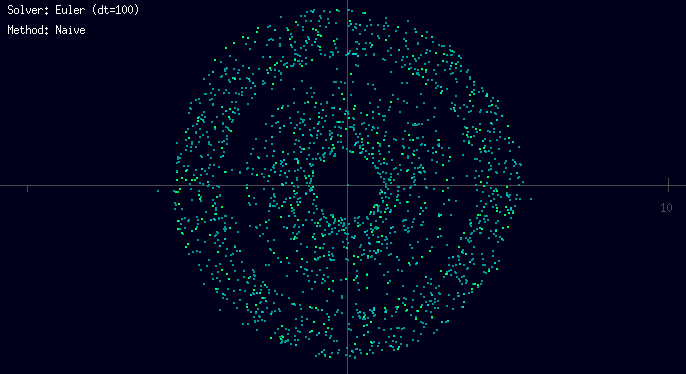
\includegraphics[scale=0.8]{images/naive.png}
\captionsetup{hypcap=false}
\captionof{figure}{Méthode naïve avec 1000 particules}
\label{fig2}
\end{center}

En terme de performance, comme prévu l'algorithme est inefficace et montre ses limites pour $N>1000$ ce qui est bien trop petit pour pouvoir simuler des galaxies.

\section{Optimisation de la méthode de calcul naïve}
\vspace{2mm}

Une première manière d'optimiser le calcul des forces est d'utiliser le principe d'action-réaction afin de ne pas effectuer plusieurs fois les calculs.
Pour cela, nous pouvons suivre une démarche d'optimisation dynamique en utilisant plus de mémoire afin de réduire nos calculs. Ainsi, si l'on considère les particules $p1$ et $p2$, lors du calcul de la force $\vec{F}_{2 \rightarrow 1}$ de $p2$ sur $p1$, nous pouvons stocker directement la force de $p1$ sur $p2$, $\vec{F}_{1 \rightarrow 2}$ qui vaut $-\vec{F}_{2 \rightarrow 1}$, ce qui nous permet de ne pas refaire le calcul lors du calcul des forces qui s'appliquent sur $p2$.

\vspace{2mm}
Cela donne donc le nombre de calculs suivant :
\vspace{1mm}

$C=\sum_{n=1}^N n = \frac{N(N-1)}{2}$

\vspace{2mm}
On peut déjà observer que la complexité de ce calcul est toujours  en $O(N^2)$ mais qu'utiliser cette méthode permet de diviser le nombre de calculs par $2$ ce qui est déjà une optimisation intéressante. Cependant, étant donné que l'on garde toujours une complexité quadratique, cela n'est toujours pas suffisamment efficace pour simuler des galaxies. En pratique, nous pouvons simuler $2000$ particules tout en ayant de bonnes performances mais au-delà de $2000$, la méthode montre ses limites.

\begin{center}
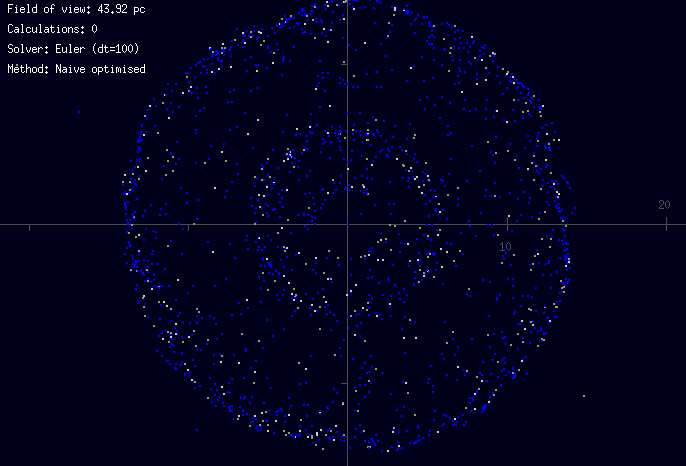
\includegraphics[scale=0.8]{images/NO.png}
\captionsetup{hypcap=false}
\captionof{figure}{Méthode naïve optimisée avec 2000 particules colorées}
\label{fig3}
\end{center} 

\section{Vérification des modèles}

Il est nécessaire de vérifier si nos modèles sont bien implémentés et cohérents avec la physique du problème. Pour cela, un moyen de procéder est de calculer l'énergie mécanique du système à partir de son énergie cinétique et de son énergie potentielle. En effet, l'énergie mécanique du système se conserve au cours du temps étant donné qu'aucune force non conservative n'est prise en compte.
Cela permet aussi de vérifier la validité de notre intégrateur car l'instabilité d'un intégrateur se traduirait par le non respect de ce principe de conservation de l'énergie mécanique.

Nos calculs ont été effectués avec un pas $\Delta t = 50 $ et $1000$ itérations.

\begin{center}
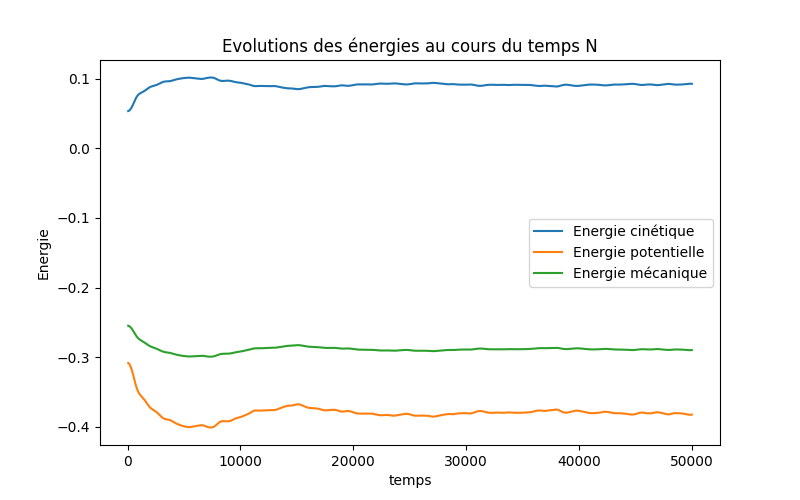
\includegraphics[scale=0.6]{resultats/Energy_N.png}
\captionsetup{hypcap=false}
\captionof{figure}{Bilan énergétique méthode naïve}
\label{fig4}
\end{center} 

\begin{center}
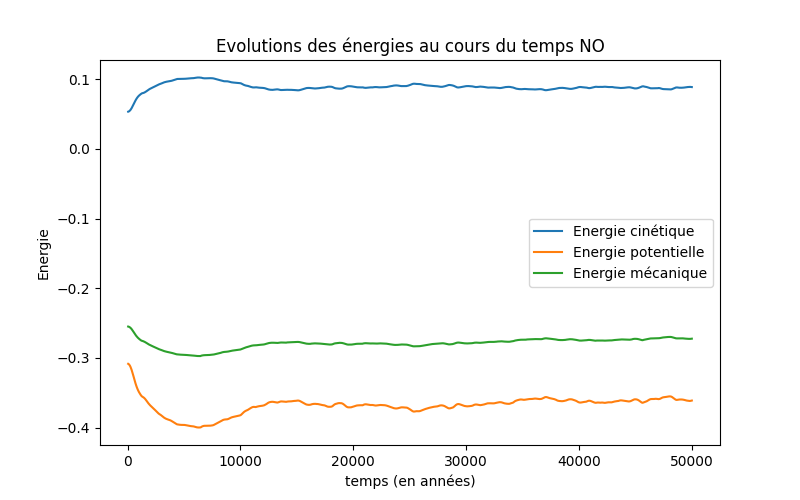
\includegraphics[scale=0.6]{resultats/Energy_NO.png}
\captionsetup{hypcap=false}
\captionof{figure}{Bilan énergétique méthode naïve optimisée}
\label{fig5}
\end{center} 


Pour les deux méthodes, au début de la simulation les énergies
varient beaucoup, cela est dû aux conditions initiales qui ne
respectent pas forcément l'aspect physique du problème.
On peut voir sur la figure $4.3$ que l'énergie mécanique de la
méthode naïve est bien constante à partir de $t=20000$, ce qui
valide bien le modèle. Cela nous informe aussi sur la vitesse de
convergence de la méthode: le modèle converge en $400$ itérations.

Sur la figure $4.4$, on peut voir que de même l'énergie mécanique
se conserve bien pour la méthode naïve optimisée à partir de la
$240$ème itération. Ainsi, la méthode converge plus vite que la 
méthode naïve.

Il est important de noter que pour les deux méthodes, on peut
observer de légère variations qui sont dues aux approximations des
modèles.